\section{Supplementary Results}

\subsection*{Programmed mapping was recovered under correct specification}

The locked implementation recovered the programmed mapping in a correctly
specified synthetic positive-control. Across five independent simulation
seeds, all five code-fixed checks passed. The locked attribute-level procedure
had a mean residual root mean squared error of 0.3522, with an empirical
five-seed 2.5th to 97.5th percentile interval of 0.3461 to 0.3647. The
corresponding residual Spearman correlation was 0.9876 (0.9848 to 0.9896).
The Food Compass baseline residual root mean squared error was 3.5411 (3.0619
to 3.8431) in the same programmed-truth experiment.

\begin{table}[t]
\caption{\textbf{Correctly specified synthetic positive-control summaries.}
Values are means and empirical 2.5th to 97.5th percentiles across five
independent simulation seeds. They are not uncertainty intervals for human
data.}
\label{tab:supp_synthetic_positive_control}
\centering
\begin{tabular}{p{0.35\textwidth} p{0.25\textwidth} p{0.25\textwidth}}
\toprule
Assignment or comparator & Residual RMSE & Residual Spearman \\
\midrule
Food Compass baseline & 3.5411 (3.0619--3.8431) & 0.0000 (0.0000--0.0000) \\
Locked attribute-level procedure & 0.3522 (0.3461--0.3647) & 0.9876 (0.9848--0.9896) \\
Random microbiome assignment & 2.8253 (2.5182--3.2532) & 0.1571 (0.0867--0.2767) \\
Sattolo-deranged assignment & 3.6541 (3.1163--4.4582) & -0.0539 (-0.2599--0.1141) \\
\bottomrule
\end{tabular}
\end{table}

\begin{figure*}[t]
\centering
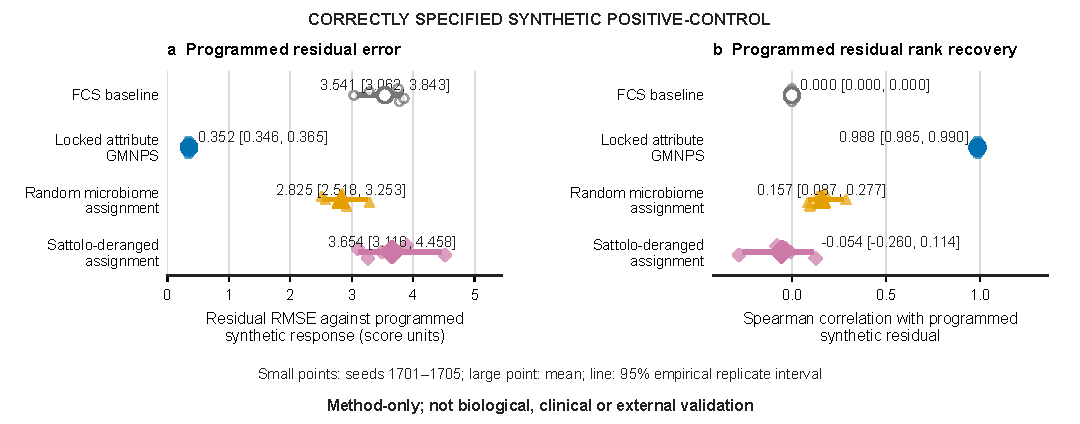
\includegraphics[width=\textwidth]{figures/supplementary_figure_S1_synthetic_positive_control.pdf}
\caption{\textbf{Correctly specified synthetic positive-control.}
\textbf{a}, Residual root-mean-square error against the programmed synthetic
response for the Food Compass baseline, locked attribute-level procedure,
random microbiome assignment and deterministic
Sattolo-deranged assignment. \textbf{b}, Spearman correlation between predicted
and programmed synthetic residuals for the same comparators. Small points
denote independent simulation seeds; large points and horizontal lines denote
the mean and empirical 2.5th--97.5th percentiles across five seeds. Each seed
comprised 24 synthetic individuals and 12 synthetic foods (288 person-food
pairs). The generator and evaluated code share the programmed mapping; the
controls belong to the same synthetic evidence family. The display assesses
numerical and assignment fidelity under correct specification only. Biological
misspecification was not assessed. Real
participant responses were not evaluated. External validity was not
established.}
\label{fig:supp_synthetic_positive_control}
\end{figure*}

Programmed-mapping recovery was lost after random or Sattolo-deranged
assignment. The random and deranged controls are parts of the same positive-
control family. The checks were fixed in the same code release and were not independently
preregistered. Because the generator uses the programmed mapping and domain
aggregation evaluated by the implementation, these findings test numerical and
assignment fidelity under correct specification. Biological misspecification
was not assessed. Real participant responses were not evaluated. External
validity was not established.

\subsection*{Combined evidence and expert-record boundary}

The fixed evidence decision remained at computational feasibility. No eligible
observed participant-by-meal outcome artifact, run-level method-lock instance,
paired metric table, prediction table, split audit or analysis-status artifact
was available. The production Food Compass and FNDDS registry also had no
approved artifact chain, and the supporting GMrepo, ZOE and knowledge-path
production registries or runs were absent.

\begin{table}[t]
\caption{\textbf{Combined evidence and expert-record boundary.} Missing
expert record classes are administrative author inputs and are not represented
as review outcomes.}
\label{tab:supp_evidence_expert_boundary}
\centering
\begin{tabular}{p{0.30\textwidth} p{0.22\textwidth} p{0.38\textwidth}}
\toprule
Evidence or record & Status & Authorized interpretation \\
\midrule
Locked attribute-level specification & Available & Computational method definition and invariants \\
Observed participant-by-meal outcomes & Unavailable & No direct-response or external-validity inference \\
Production 9,234-food run & Not executed & No population preservation, transition or heterogeneity inference \\
Correctly specified synthetic positive-control & Available & Implementation fidelity under programmed correct specification \\
Registry-bound GMrepo run & Not executed & No person-level generalization or disease result \\
Registry-bound ZOE rank run & Not executed & No aggregate rank-concordance result \\
Registry-bound knowledge-path run & Not executed & No biological or mechanistic validation result \\
External C1 feedback workbooks & Available and hash bound & Qualitative nutrient-channel content review \\
Anonymous item-level C3 records & AUTHOR\_INPUT\_NEEDED & No consensus percentage or final-passage claim \\
Anonymous item-level E4 records & AUTHOR\_INPUT\_NEEDED & No clinical-readiness or translation verdict \\
Exact reviewer denominator & Not established & No exact expert-count claim \\
\bottomrule
\end{tabular}
\end{table}

\subsection*{Available expert records supported content review only}

Available expert feedback informed the treatment of carbohydrate, zinc, copper
and vitamin A as retinol activity equivalents. The available evidence supports
qualitative content review only; the combined evidence and expert-record
boundary is reported in Supplementary Table S3.
